\chapter{Resultados}\label{cap:resultados}

Após análise das ferramentas estudadas e posteriormente eleitas as que melhores se adequaram ao presente estudo, partiu-se para a elaboração e concepção do modelo proposto para entrega de aplicação externa com base em uma visão DevOps.

A figura 5 representa a proposta de modelo de arquitetura para aplicação externa pretendida nesse estudo. O processo que dará início à sequencia de testes e deploy, começará com a requisição do usuário (desenvolvedor) para adquirir um repositório com intuito de armazenar uma determinada aplicação web. Isso quer dizer, que o programador terá acesso a um formulário de requisição (via sistema web) para armazenamento do seu código e após analisado, será retornado ao mesmo o link desse repositório a fim de que o mesmo possa hospedar a sua aplicação. Os códigos e alterações serão enviados ao GitHub. Depois de enviar o código, o Jenkins receberá continuamente os códigos e executará os testes. Sendo os testes realizados com sucesso e tendo retorno positivo, sem erros, o Jenkins realizará o deploy no servidor através do Docker.

\begin{figure} [htb]
	\centering
	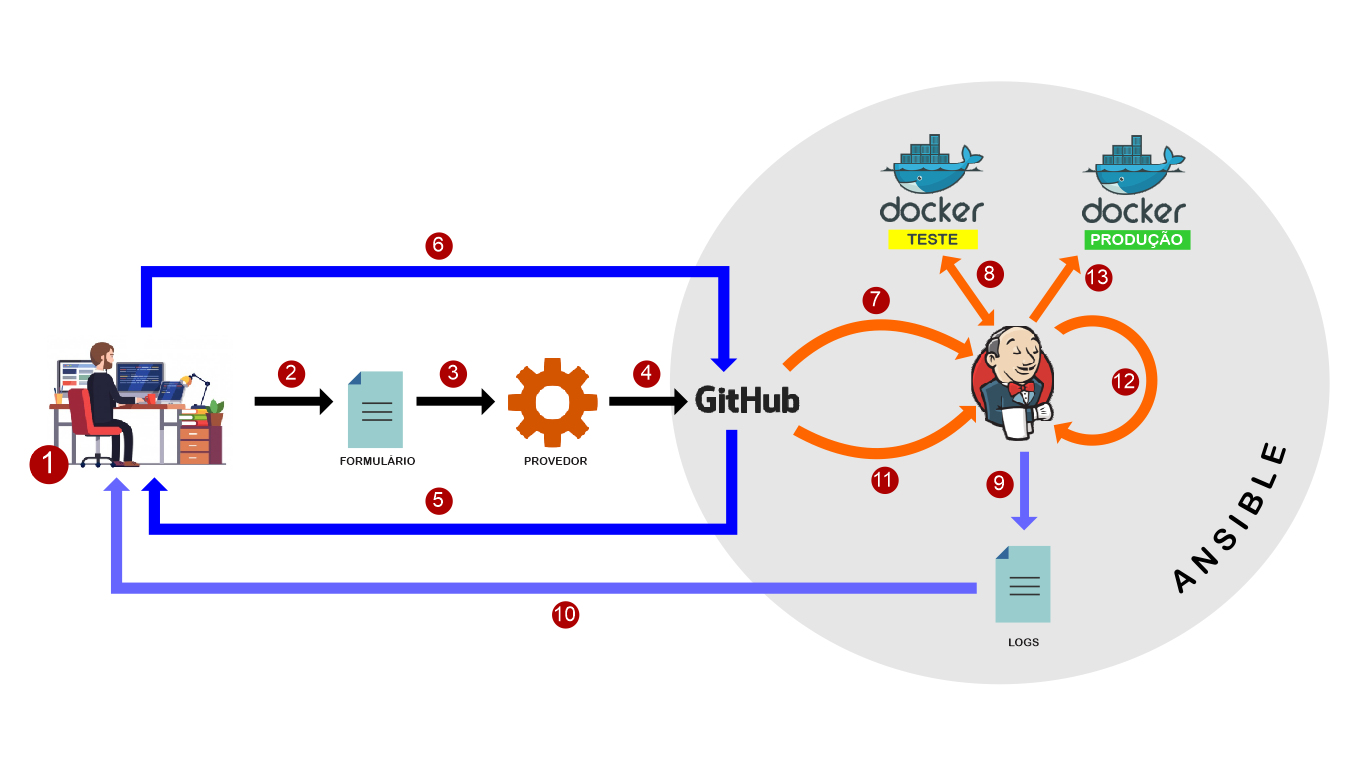
\includegraphics[width=1.05\linewidth]{imagens/MODELODEPLOY}
\caption{Representação da Arquitetura Proposta}
Fonte: Acervo próprio
	\label{fig:modelodeploy}
\end{figure}


Considerando o modelo apresentado na figura 5, temos como sequenciamento mais detalhado, as etapas a seguir, absorvendo desde o início de uma requisição até a disponibilização da aplicação em servidor de produção.

\begin{enumerate}
	\item No ponto de partida, é pre-requisito a existência de conteúdo codificado em linguagem de programação, que permita o versionamento do projeto.
	\item O desenvolvedor faz a requisição de um novo repositório através de um formulário, que contenha as informações pertinentes, tais como, chave ssh, membros do projeto e nome do mesmo;
	\item A requisição é recebida pelo provedor que verifica os dados de solicitação, avalia a disponibilidade de repositório;
	\item O provedor valida a disponibilidade e cria um novo repositório no GitHub;
	\item O link do repositório é retornado ao usuário juntamente com sua chave de autenticação;
	\item O desenvolvedor envia os commits e o GitHub gera uma notificação de alteração ao Jenkins;
	\item Jenkins recebe a notificação (Git Fetch – Git Merge – Templates Ansible – Dry Run – Commit Check);
	\item O Jenkins realiza teste jundo ao contêiner Docker destinado para tanto;
	\item Jenkins gera um histórico (Notificação aos Administradores);
	\item Administrador analisa os logs de testes;
	\item GitHub gera nova notificação ao Jenkins;
	\item Jenkins gera novo release e gera nova tag de versão;
	\item Estando as alterações aprovadas o Jenkins realiza deploy da aplicação em um contêiner Docker destinado a produção;
\end{enumerate}
















